%\begin{figure}[h]
\label{retwX}
  \centering
  \begin{minipage}[t]{\linewidth}
      \begin{tikzpicture}[scale=0.9]
\begin{axis}[
    width=\columnwidth,
    height=0.3\textheight,
    xlabel={Neuro-Matching Threshold ($\tau_m$)},
    ylabel={Accuracy},
    title={Performance with the ANLI dataset},
    grid=major,
    legend style={at={(0.5,-0.25)}, anchor=north, legend columns=3},
    ymin=0.45,
    ymax=0.75,
    xtick={0.5,0.55,0.6,0.65,0.7,0.75,0.8,0.85,0.9,0.95,1.0},
    ymajorgrids=true,
    major grid style={line width=0.1pt,draw=gray!30},
]

% original Data - Accuracy, tau_c=80
\addplot[color=blue, mark=*, thick] coordinates {
    (0.5,0.510000) (0.55,0.516667) (0.6,0.486667) (0.65,0.493333) (0.7,0.503333) (0.75,0.500000) (0.8,0.500000) (0.85,0.500000) (0.9,0.500000) (0.95,0.500000) (1,0.500000)
};

% original Data - Accuracy, tau_c=90
\addplot[color=blue, mark=square*, thick] coordinates {
    (0.5,0.513333) (0.55,0.503333) (0.6,0.486667) (0.65,0.493333) (0.7,0.506667) (0.75,0.500000) (0.8,0.500000) (0.85,0.500000) (0.9,0.500000) (0.95,0.500000) (1,0.500000)
};

% original Data - Accuracy, tau_c=100
\addplot[color=blue, mark=triangle*, thick] coordinates {
    (0.5,0.513333) (0.55,0.506667) (0.6,0.500000) (0.65,0.503333) (0.7,0.506667) (0.75,0.496667) (0.8,0.500000) (0.85,0.500000) (0.9,0.500000) (0.95,0.500000) (1,0.500000)
};

% 1-step Data - Accuracy, tau_c=80
\addplot[color=orange, mark=*, thick] coordinates {
    (0.5,0.620000) (0.55,0.636667) (0.6,0.643333) (0.65,0.603333) (0.7,0.550000) (0.75,0.523333) (0.8,0.513333) (0.85,0.506667) (0.9,0.500000) (0.95,0.500000) (1,0.500000)
};

% 1-step Data - Accuracy, tau_c=90
\addplot[color=orange, mark=square*, thick] coordinates {
    (0.5,0.623333) (0.55,0.633333) (0.6,0.653333) (0.65,0.610000) (0.7,0.553333) (0.75,0.523333) (0.8,0.513333) (0.85,0.506667) (0.9,0.500000) (0.95,0.500000) (1,0.500000)
};

% 1-step Data - Accuracy, tau_c=100
\addplot[color=orange, mark=triangle*, thick] coordinates {
    (0.5,0.570000) (0.55,0.596667) (0.6,0.616667) (0.65,0.603333) (0.7,0.550000) (0.75,0.520000) (0.8,0.513333) (0.85,0.506667) (0.9,0.500000) (0.95,0.500000) (1,0.500000)
};

% 2-step Data - Accuracy, tau_c=80
\addplot[color=red, mark=*, thick] coordinates {
    (0.5,0.680000) (0.55,0.683333) (0.6,0.676667) (0.65,0.613333) (0.7,0.563333) (0.75,0.530000) (0.8,0.513333) (0.85,0.510000) (0.9,0.506667) (0.95,0.503333) (1,0.503333)
};

% 2-step Data - Accuracy, tau_c=90
\addplot[color=red, mark=square*, thick] coordinates {
    (0.5,0.670000) (0.55,0.676667) (0.6,0.670000) (0.65,0.613333) (0.7,0.556667) (0.75,0.526667) (0.8,0.513333) (0.85,0.510000) (0.9,0.506667) (0.95,0.503333) (1,0.503333)
};

% 2-step Data - Accuracy, tau_c=100
\addplot[color=red, mark=triangle*, thick] coordinates {
    (0.5,0.570000) (0.55,0.626667) (0.6,0.680000) (0.65,0.633333) (0.7,0.580000) (0.75,0.533333) (0.8,0.520000) (0.85,0.510000) (0.9,0.506667) (0.95,0.503333) (1,0.503333)
};

% 3-step Data - Accuracy, tau_c=80
\addplot[color=green, mark=*, thick] coordinates {
    (0.5,0.703333) (0.55,0.713333) (0.6,0.703333) (0.65,0.666667) (0.7,0.600000) (0.75,0.536667) (0.8,0.520000) (0.85,0.506667) (0.9,0.510000) (0.95,0.510000) (1,0.506667)
};

% 3-step Data - Accuracy, tau_c=90
\addplot[color=green, mark=square*, thick] coordinates {
    (0.5,0.696667) (0.55,0.713333) (0.6,0.700000) (0.65,0.660000) (0.7,0.603333) (0.75,0.540000) (0.8,0.520000) (0.85,0.506667) (0.9,0.510000) (0.95,0.510000) (1,0.506667)
};

% 3-step Data - Accuracy, tau_c=100
\addplot[color=green, mark=triangle*, thick] coordinates {
    (0.5,0.566667) (0.55,0.643333) (0.6,0.653333) (0.65,0.676667) (0.7,0.596667) (0.75,0.546667) (0.8,0.516667) (0.85,0.506667) (0.9,0.510000) (0.95,0.510000) (1,0.506667)
};

\end{axis}
\end{tikzpicture}
  \end{minipage}
  \begin{minipage}[t]{\linewidth}
      \begin{tikzpicture}[scale=0.9]
\begin{axis}[
    width=\columnwidth,
    height=0.3\textheight,
    xlabel={Neuro-Matching Threshold ($\tau_m$)},
    ylabel={Accuracy},
    title={Performance with the ARCT dataset},
    grid=major,
    legend style={at={(0.5,-0.25)}, anchor=north, legend columns=2},
    ymin=0.45,
    ymax=0.75,
    xtick={0.5,0.55,0.6,0.65,0.7,0.75,0.8,0.85,0.9,0.95,1.0},
    ymajorgrids=true,
    major grid style={line width=0.1pt,draw=gray!30},
]

% original Data - Accuracy, tau_c=80
\addplot[color=blue, mark=*, thick] coordinates {
    (0.5,0.527273) (0.55,0.516667) (0.6,0.510204) (0.65,0.506667) (0.7,0.513333) (0.75,0.513333) (0.8,0.500000) (0.85,0.500000) (0.9,0.500000) (0.95,0.500000) (1,0.500000)
};
\addlegendentry{original ($\tau_c=80$)}

% original Data - Accuracy, tau_c=90
\addplot[color=blue, mark=square*, thick] coordinates {
    (0.5,0.533058) (0.55,0.522901) (0.6,0.516667) (0.65,0.503333) (0.7,0.516667) (0.75,0.513333) (0.8,0.500000) (0.85,0.500000) (0.9,0.500000) (0.95,0.500000) (1,0.500000)
};
\addlegendentry{original ($\tau_c=90$)}

% original Data - Accuracy, tau_c=100
\addplot[color=blue, mark=triangle*, thick] coordinates {
    (0.5,0.496667) (0.55,0.496667) (0.6,0.506667) (0.65,0.503333) (0.7,0.503333) (0.75,0.496667) (0.8,0.500000) (0.85,0.500000) (0.9,0.500000) (0.95,0.500000) (1,0.500000)
};
\addlegendentry{original ($\tau_c=100$)}

% 1-step Data - Accuracy, tau_c=80
\addplot[color=orange, mark=*, thick] coordinates {
    (0.5,0.580000) (0.55,0.583333) (0.6,0.596667) (0.65,0.606667) (0.7,0.606667) (0.75,0.573333) (0.8,0.546667) (0.85,0.526667) (0.9,0.506667) (0.95,0.503333) (1,0.503333)
};
\addlegendentry{1-step ($\tau_c=80$)}

% 1-step Data - Accuracy, tau_c=90
\addplot[color=orange, mark=square*, thick] coordinates {
    (0.5,0.593333) (0.55,0.593333) (0.6,0.606667) (0.65,0.623333) (0.7,0.620000) (0.75,0.580000) (0.8,0.546667) (0.85,0.530000) (0.9,0.506667) (0.95,0.503333) (1,0.503333)
};
\addlegendentry{1-step ($\tau_c=90$)}

% 1-step Data - Accuracy, tau_c=100
\addplot[color=orange, mark=triangle*, thick] coordinates {
    (0.5,0.556667) (0.55,0.556667) (0.6,0.553333) (0.65,0.566667) (0.7,0.573333) (0.75,0.540000) (0.8,0.516667) (0.85,0.516667) (0.9,0.506667) (0.95,0.503333) (1,0.503333)
};
\addlegendentry{1-step ($\tau_c=100$)}

% 2-step Data - Accuracy, tau_c=80
\addplot[color=red, mark=*, thick] coordinates {
    (0.5,0.584821) (0.55,0.592437) (0.6,0.602740) (0.65,0.613333) (0.7,0.606667) (0.75,0.600000) (0.8,0.573333) (0.85,0.536667) (0.9,0.503333) (0.95,0.503333) (1,0.503333)
};
\addlegendentry{2-step ($\tau_c=80$)}

% 2-step Data - Accuracy, tau_c=90
\addplot[color=red, mark=square*, thick] coordinates {
    (0.5,0.599174) (0.55,0.604651) (0.6,0.620000) (0.65,0.623333) (0.7,0.613333) (0.75,0.600000) (0.8,0.573333) (0.85,0.536667) (0.9,0.503333) (0.95,0.503333) (1,0.503333)
};
\addlegendentry{2-step ($\tau_c=90$)}

% 2-step Data - Accuracy, tau_c=100
\addplot[color=red, mark=triangle*, thick] coordinates {
    (0.5,0.540000) (0.55,0.533333) (0.6,0.570000) (0.65,0.580000) (0.7,0.576667) (0.75,0.563333) (0.8,0.546667) (0.85,0.520000) (0.9,0.503333) (0.95,0.503333) (1,0.503333)
};
\addlegendentry{2-step ($\tau_c=100$)}

% 3-step Data - Accuracy, tau_c=80
\addplot[color=green, mark=*, thick] coordinates {
    (0.5,0.621622) (0.55,0.634454) (0.6,0.650000) (0.65,0.646667) (0.7,0.656667) (0.75,0.636667) (0.8,0.616667) (0.85,0.563333) (0.9,0.520000) (0.95,0.513333) (1,0.513333)
};
\addlegendentry{3-step ($\tau_c=80$)}

% 3-step Data - Accuracy, tau_c=90
\addplot[color=green, mark=square*, thick] coordinates {
    (0.5,0.632231) (0.55,0.643411) (0.6,0.660000) (0.65,0.656667) (0.7,0.653333) (0.75,0.633333) (0.8,0.613333) (0.85,0.563333) (0.9,0.520000) (0.95,0.513333) (1,0.513333)
};
\addlegendentry{3-step ($\tau_c=90$)}

% 3-step Data - Accuracy, tau_c=100
\addplot[color=green, mark=triangle*, thick] coordinates {
    (0.5,0.543333) (0.55,0.556667) (0.6,0.566667) (0.65,0.583333) (0.7,0.610000) (0.75,0.593333) (0.8,0.563333) (0.85,0.540000) (0.9,0.520000) (0.95,0.513333) (1,0.513333)
};
\addlegendentry{3-step ($\tau_c=100$)}

\end{axis}
\end{tikzpicture}
  \end{minipage}
  \caption{Overall accuracy (entailment and non-entailment) for different options for the implicit premises for the ANLI and ARCT datasets. Original means using the helpful/unhelpful intermediate premises given in the dataset, and 1- (resp. 2- and 3-) step means using the response from prompting the LLM for one (resp. two and three) steps of helpful/unhelpful intermediate premises.}
  \label{anlifig}
%\end{figure}
